\subsection{Historical Preliminaries}

The history of phase retrieval cannot be told without making mention of x-ray crystallography, the field that first brought scientific interest to this problem and by many metrics its most decorated and fruitful application.  In x-ray crystallography, the goal is to gain an image of the positions of atoms within a molecule by illuminating a crystallized sample with x-rays.  The molecular structure is deduced from the pattern of the radiation diffracted by the sample.  A rough diagram of this setup is shown in figure \ref{fig:xray_cryst}.

\begin{figure}
  \centering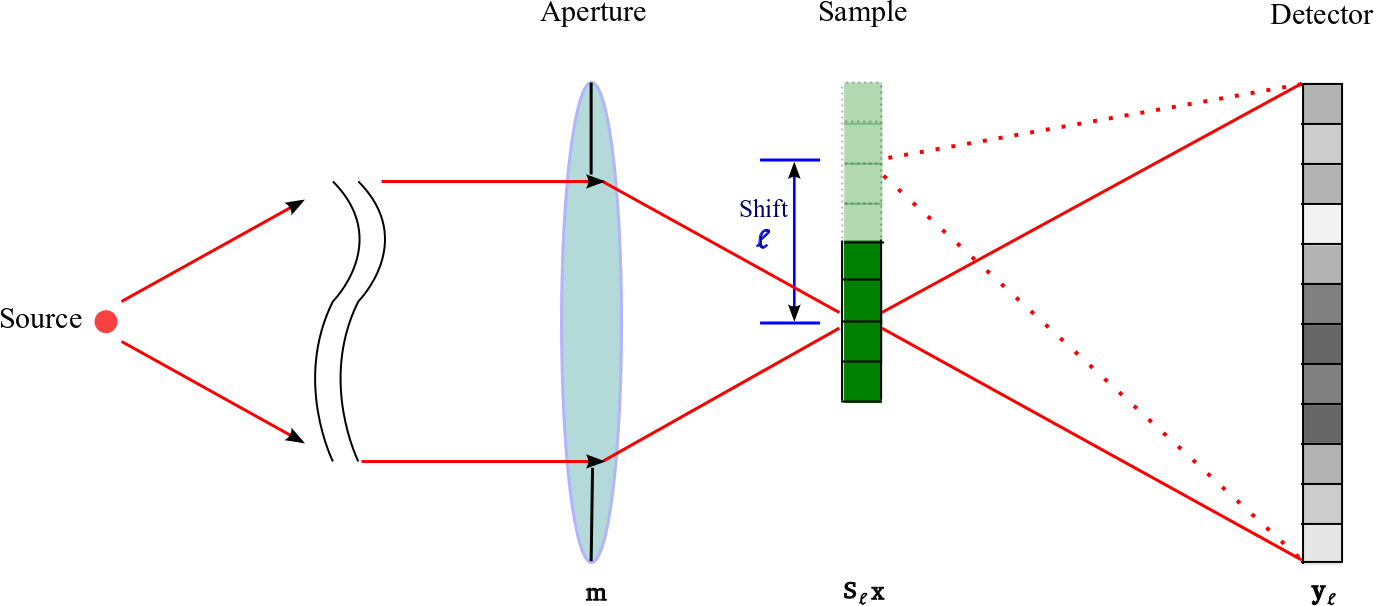
\includegraphics[scale=0.25]{pics/ptych1D}
  \caption[Experimental setup for x-ray crystallography]
          {Experimental setup for x-ray crystallography.   {\small
              (Adapted from ``Fly-scan ptychography'', Huang et al.,
              Scientific Reports 5 (9074), 2015.)}}
  \label{fig:xray_cryst}
\end{figure}

This seemingly simple technique has been indispensable for the study of chemistry, biology, and physics, having been used to confirm or identify the arrangements of atoms in a wide variety of important compounds.  Over a dozen discoveries made through x-ray crystallography -- or made in developing the technique -- have been recognized by Nobel Prizes in Physics, Chemistry, and Medicine or Physiology.  Indeed, the first Nobel Prize in Physics was awarded to Wilhelm R\"ontgen in 1901 for his discovery of x-rays.  The 1914 Prize in Physics was conferred upon Max von Laue for discovering the diffraction of x-rays by atomic crystals, and in 1915 William and Lawrence Bragg earned the same distinction for performing the first complete characterizations of atomic crystal structures \cite{galli2014nobel}.  Since the time of these highly esteemed pioneering discoveries, x-ray crystallography has been used to produce accurate molecular models of a number of drugs (e.g., \cite{cell2001antibios, rasmussen2007adrenergic, schindler2000kinase}), including penicillin in Dorothy Crowfoot Hodgkin's Nobel prize-winning work in 1963 \cite{hodgkin1963penicillin}.  It has elucidated several human biological compounds, including innumerable proteins \cite{kimber2003protein, varsani1993isomerase} and human DNA, for whose analysis in 1953 James Watson, Maurice Wilkins, and Francis Crick were awarded the Nobel prize in 1962, relying on the crystallographic images of Rosalind Franklin \cite{franklin1953nature,watson1962nobel_lecture,watson1953nature,wilkins1953nature}.  And this technology remains extremely relevant today, playing an active role in material sciences, where crystallography is being used to characterize the degradation of lithium-ion batteries \cite{hausbrand2015battery, andrej2018battery} and to study carbon nanostructures such as fullerenes \cite{lamb1990carbon, kroto1985fullerene}, whose analysis earned the 1996 Nobel Prize in Chemistry \cite{galli2014nobel}.

With such a history, x-ray crystallography is an essential application of phase retrieval, and it is %% a worthy diversion %% imperative %% worth taking the time %% useful
informative to state its mathematical formulation in this dissertation.

\subsection{Mathematical Model}

\subsection{Diffraction as a Fourier transform}
We begin by considering the mechanism of diffraction of waves.  

